% file: reasoning_case.tex

\begin{ReasoningBox}[title=Comparative Analysis] % 可以通过 title 参数修改标题
    % --- 第一部分：问题描述与图片 ---
    % \begin{minipage}[t]{0.58\textwidth}
    \begin{wrapfigure}{r}{0.3\textwidth}
        \centering
        % wrapfigure 通常顶部会有多余空白，使用负 vspace 向上提，让图片和第一行文字对齐
        \vspace{-30pt} 
        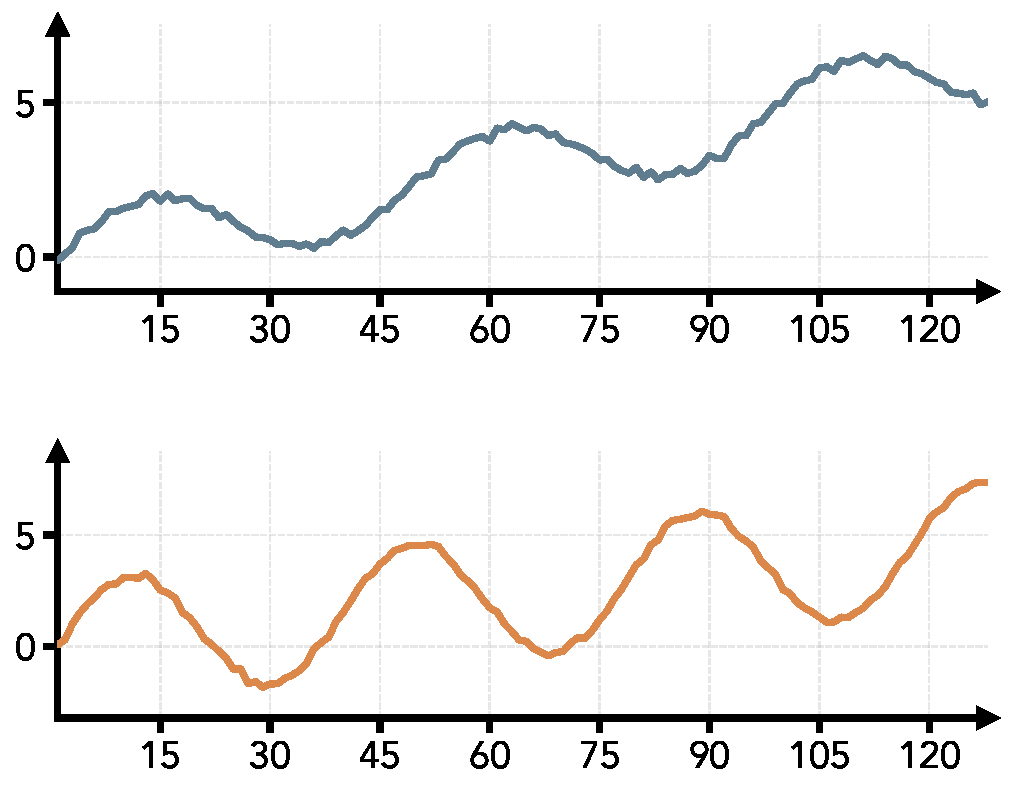
\includegraphics[width=\linewidth]{blocks/sample_cases_success/similarity.pdf}
        % 调整底部的留白
        \vspace{-20pt}
    \end{wrapfigure}
        \textbf{Question:} You are given two time series that both have a trend component. Do they share the same direction of trend?

    \vspace{1.5em}

    % --- 第二部分：选项 ---
    \textbf{Answer Choices:} \\ (A) Yes \\ (B) No \\
    \textbf{Correct Answer:} \textcolor{correctgreen}{(A)} \\
\end{ReasoningBox}